
\documentclass[12pt]{article}

% =================================
% PACKAGES ========================
% =================================

\usepackage[top=2.5cm, bottom=2.5cm, left=2.5cm, right=2.5cm, headheight = 15pt]{geometry}

% Set-up commands
\usepackage[T1]{fontenc}
\usepackage[utf8]{inputenc}
\usepackage{lmodern}
\usepackage[english]{babel}
\usepackage[autostyle]{csquotes}
\usepackage{textcomp}

% Better text
\usepackage{ragged2e} %text alignment
\usepackage{xcolor}   %colors
\usepackage{enumitem} %better control over lists
\usepackage{fancyhdr} %nice headers at tops of pages

% Better Tables
\usepackage{tabularx} %alignments
\usepackage{booktabs} %toprule, midrule, etc.
\newcolumntype{L}{>{\RaggedRight}X} %new column (fixed width, left aligned)
\newcolumntype{R}{>{\RaggedLeft}X} %new column (fixed width, right aligned)

% Better Figures
\usepackage{graphicx} %figures
\usepackage{pdfpages} %insert whole pdf as a page
\usepackage{float}

% Better Commands
\usepackage{xspace} %allow commands to detect punctuation
\usepackage[version=4]{mhchem} %chemistry

% Better Navigation
\usepackage{hyperref} %clickable links
\AtBeginDocument{\def\chapterautorefname{Chapter}} %Capitalise "chapter" in \autoref
\AtBeginDocument{\def\sectionautorefname{Section}} %Capitalise "section" in \autoref
\AtBeginDocument{\def\subsectionautorefname{Subsection}} %Capitalise "subsection" in \autoref

% Better Captions
\usepackage[font=small,labelfont=bf]{caption} % make caption labels bold and a bit smaller

% Better Code
\usepackage{listings} 
\usepackage{pythonhighlight}% For formatted code blocks

% Only for template
\usepackage{mwe}
\usepackage{lipsum}
\usepackage{blindtext}

% Set-up References
%\usepackage[
%   backend = biber, 
%   natbib = true,
%   style = numeric-comp,
%   sorting = none,
%   url = true,
%   isbn = false,
%   uniquename = false,
%   maxcitenames = 1,
%   maxbibnames = 99,
%   date = year,
%   giveninits = true
% ]{biblatex} % nice defaults

% \DeclareNameAlias{author}{family-given}
% \renewbibmacro{in:}{}

% \addbibresource{ref.bib} % add your own bib resources if needed
\usepackage[style=authoryear-ibid,backend=biber]{biblatex}

\addbibresource{MChem_refs.bib}


% Set-up Colours
\definecolor{mygray}{gray}{0.7}
\definecolor{airforceblue}{rgb}{0.36, 0.54, 0.66}

\hypersetup{
  colorlinks = true,
  urlcolor = airforceblue, 
  citecolor = airforceblue, 
  linkcolor = airforceblue
}

% Formatting of code blocks
\definecolor{green_comment}{rgb}{0,0.6,0}

\lstset{
  language = R,
  basicstyle = \footnotesize,
  commentstyle = \color{green_comment},
  frame = single,
  numbers = left
}

% =================================
% COMMANDS ========================
% =================================

% chemistry
\newcommand{\nox}{\ce{NO_{x}}\xspace}
\newcommand{\notwo}{\ce{NO2}\xspace} 
\newcommand{\cotwo}{\ce{CO2}\xspace}
\newcommand{\ammonia}{\ce{NH3}\xspace}

% units
\newcommand{\gkg}{g~kg\textsuperscript{-1}\xspace}
\newcommand{\gkm}{g~km\textsuperscript{-1}\xspace}

% =================================
% META ============================
% =================================

\newcommand{\thesistitle}{Methane emission flux estimation from offshore oil and gas platforms with a dispersion model and airborne measurements.}

\title{
    \textbf{\thesistitle} \\~\\
    \large Interim Report 
    }
\author{Irene Monreal Campos}

% =================================
% DOCUMENT ========================
% =================================

% title page & contents
\begin{document}
\maketitle
\begin{figure}[bht]
    \centering
    
\includegraphics[width=.7\linewidth]{Plots/York Logo.png}
\end{figure}
\tableofcontents
\bigskip
\newpage

% start fancy headers
\pagestyle{fancy}
\rhead{\slshape\nouppercase{\leftmark}}
\lhead[E,O]{}

% overview section
\begin{abstract}
The oil and gas industry accounts for 22\% of global methane emissions\parencite{Saunois2020The20002017}, however accurate quantification of methane emission fluxes from this sector remains technically challenging. Top-down quantification methods have encountered issues associated with atmospheric boundary layer dynamics, and the presence of multiple overlapping emission sources.
In this study, we estimate methane emission fluxes from the uncontrolled gas release at the Total Elgin offshore platform in 2012 using airborne measurements from mission B689 by the FAAM Airborne Laboratory, and atmospheric dispersion modelling with ADMS 6. By adopting a novel emission ratio approach instead of the widely published mass balance methodology, we estimate an emission flux of $48\pm6$ g/s. 
We describe the method which involves running ADMS with a known emission flux and scaling the model outputs to match observed methane enhancements. 
A sensitivity analysis highlights the importance of source characterisation, boundary layer conditions, wind profiles treatment, and the need to adopt a marine boundary layer scheme when dealing with off-shore conditions. 
After optimising the ADMS model setup, our derived emission flux differed by a factor of 10 from published flux values derived using mass balance methodologies. The most likely explanation is the overestimation of the source volume, indicating the need for further investigation.

\end{abstract}

\renewcommand{\abstractname}{Acknowledgements}
\newpage\begin{abstract}
A big thank you to Steph and Patryk for being great teachers and supervisors, for believing in me and offering incredible opportunities, for answering all my questions, for the lengthy discussions about science (among other things) and for the almost unlimited supply of coffee, digestives and pastries without which I would not have survived the year. 

To Eleanor, Alex, Jack, Olivia and Steven, for putting up with my pop culture references all year, for taking me to swim so that I stay sane and for making FAAM a fun place to be. To Dave, for answering  all my coding questions, and for being an amazing running partner. To Annalisa, for always checking that I was ok and for feeding me through the year. To all staff from FAAM,  Airtask and Avalon for having made this year an incredible placement. 

  To my family: Mum, Dad and Sara, thank you for always being there when I need you and for being an endless source of support. To my grandparents, especially to my grandad Jesús. Gracias por apoyarme incondicionalmente, prestar tanto interés en todo lo que hago y por siempre creer en mí. El orgullo que siempre muestras hacia mis logros, pequeños o grandes, es mi gran fuente de motivación.


\end{abstract}

\newpage\section{Introduction}\label{intro}
Methane is the second largest contributor to climate change,  with a radiative forcing effect of 0.5 Wm\textsuperscript{-2} \parencite{Prather2001AtmosphericGases} linked to human activity since the pre-industrial era. On a 20-year timescale, methane’s warming potential is 84 times more potent than carbon dioxide \parencite{Myhre2013AnthropogenicForcing}.   

Currently, the oil and gas sector is estimated to contribute to 22\% of global methane emissions \parencite{Saunois2020The20002017}, however, this value is associated with large uncertainties, as many unexpected processes can lead to large releases to the atmosphere like flaring, cold venting, or uncontrolled methane release accidents. Methane has been addressed as a major climate change problem, and many mitigation strategies have been put in place. Most recently, in the COP27 Global Methane Pledge, aiming for a 30\% reduction of methane emissions by 2023\parencite{IEA2022Global2022}. For this reason, accurate quantification of methane is essential. 

This study focuses on offshore oil and gas facilities. Their emissions have historically been under reported due to the bottom-up methodology commonly used.  It relies on theoretical estimations and there is a large potential for systematic errors.  One way to improve bottom-up emission calculations is by direct atmospheric measurements (top-down approach).  The UN Environment Programme (UNEP) launched the International Methane Emissions Observatory (IMEO) in 2022 to provide top-down emissions data, to enable over 80 oil and gas companies and governments across the globe to target strategic mitigation action. There have been several studies performed using top-down approaches in the offshore oil and gas sector, repeatedly showing that bottom-up derived methane emissions have been under reported \parencite{GorchovNegron2020AirborneMexico}.

However, accurately quantifying methane emission fluxes from the oil and gas sector with a top-down approach remains challenging. Previous methods can encounter issues associated with atmospheric boundary layer dynamics, and the presence of multiple overlapping emission sources. 

To address this problem, we evaluate a methodology to estimate methane emission fluxes using the commercially available dispersion model ADMS 6 and aircraft measurements of meteorology and plume concentrations.  It considers many parameters including meteorology variables such as boundary layer conditions stability and high-accuracy atmospheric dynamics measurements from the aircraft. Assumptions about the source type are also investigated needed for accurately simulating plume dispersion behaviour.

The ADMS model setup for this calculation  uses single-modelled plume concentration enhancements with a fixed mass flux input which is then scaled using the ratio between the co-located modelled and observed enhancements. 

We evaluate this proposed methodology using  a case study flown by the FAAM Airborne Laboratory (FAAM). The study focuses on the TOTAL Elgin gas platform accidental methane release in 2012 \parencite{Lee2018FlowRelease}. 

The Elgin gas field is located in the Central Graben of the UK North Sea, situated approximately 240 km east of Aberdeen (Figure 1).

\begin{figure}[H]
\centering
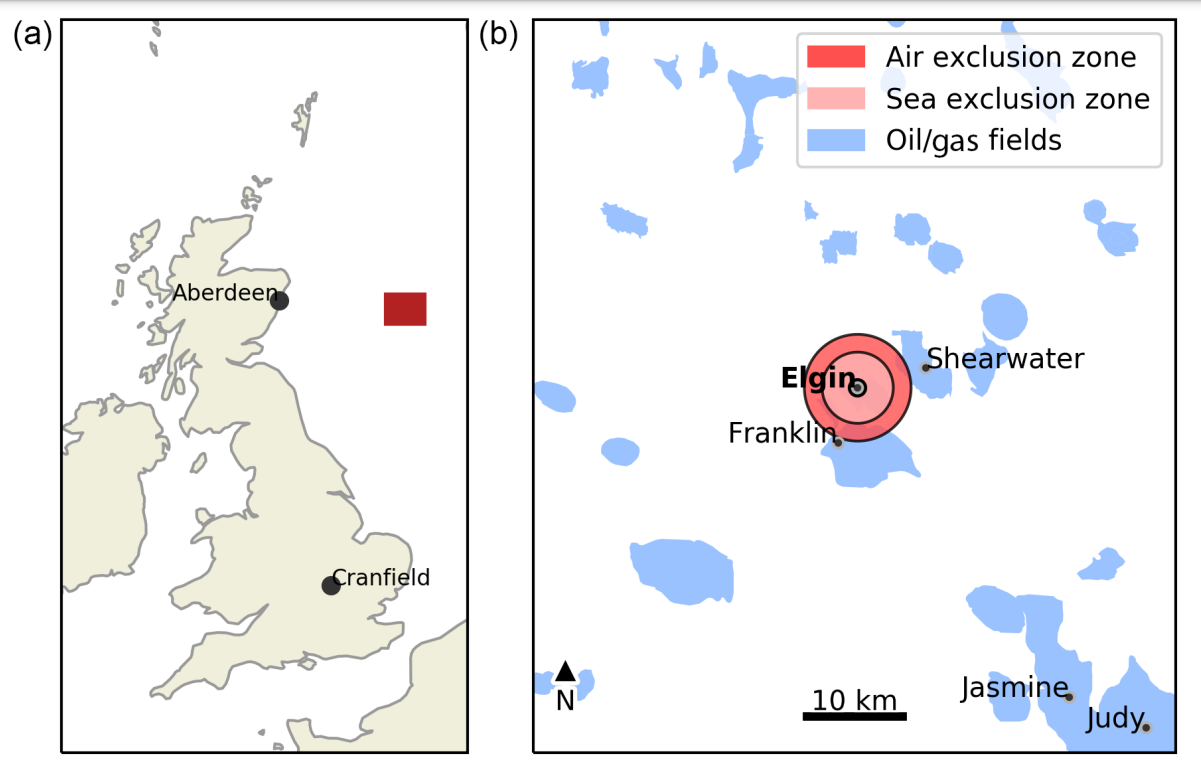
\includegraphics[width=0.8\textwidth]{Plots/elginmap.png}
\caption{\label{fig:elgin}} "Map showing the location and details of the Elgin fieldand platform. Panel (a) shows the location of the field in the North Sea, with the red rectangle shown on panel (b). The black dot indicates the location of the Elgin platform with the grey dots showing
the location of neighbouring platforms."\parencite[]{Lee2018FlowRelease}.
 
\end{figure}


On 25 March 2012, an accidental and uncontrolled hydrocarbon release took place at the 22/30c-G4 well, which accesses the Elgin reservoir at a depth of around 5.5 km. This incident led to the abandonment of the Elgin Process, Utilities and Quarters (PUQ) platform and the evacuation of non-essential personnel from nearby installations. The actions taken in response to this event resulted in the shutdown or disruption of nearly 10\% of the UK's natural gas supply for 6–7 weeks, with the well finally being capped on 16 May 2012.
The Elgin gas well is known for producing both natural gas, primarily methane, and natural gas condensate (Fort and Senequier, 2003). Given the presence of condensate and gas, concerns regarding potential fuel and air explosions arose.  Consequently, remote methods were pursued, and an aerial survey was considered appropriate due to its ability to limit the duration and concentration of human exposure to the plume.
In response, within five days of the platform's abandonment, FAAM deployed its chemically instrumented BAe-146 research aircraft to measure the gas plume resulting from the release.

The results from the calculated flux in this study  are compared with the flux values determined with the more established mass-balance methodology\parencite{Lee2018FlowRelease} and sources of uncertainties are discussed.


\newpage\section{Methods}\label{methods}

\subsection{Emission ratios and mass balance methodology}

We adopt an emission ratio  approach to estimate the emission flux rates from off-shore platforms, as opposed to the mass balance methodologies used in \cite{Lee2018FlowRelease}.

The mass balance methodology implies a series of mathematical equations to calculate the emission mass flux using the measured plume 3D dispersion  extent, wind speed and observed pollutant concentration enhancement above background.  It assumes a Gaussian plume dispersion, vertical mixing below the boundary layer top and stable meteorological conditions. Mass balance methodology can also take into consideration the effect of different boundary layer heights, accounting for vertical mixing (Figure 2). 
\begin{figure}[H]
\centering
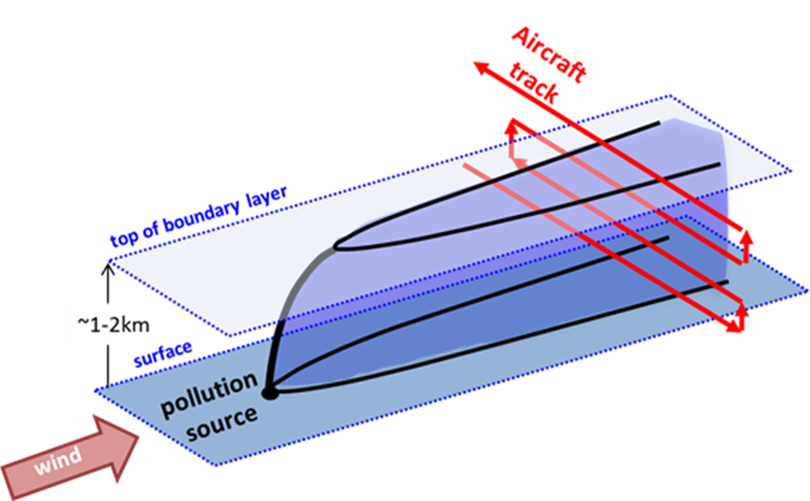
\includegraphics[width=0.8\textwidth]{Plots/Mass balance.png}
\caption{\label{fig:mass balance}} Schematic view of mass balance transects. Credit: Alina Fiehn, Institut für Physik der Atmosphäre, DLR. 
\end{figure}

The emission ratio approach used in this study involves modelling a single plume dispersion with a known emission flux, and then rationing the observations and model outputs to calculate the emission flux from the sampled source. This methodology provides a way of overcoming the limitations of observation scarcity and/or taking into account the uncertainties of more complex dispersion parameters such as boundary layer stability \parencite[]{Shah2020TestingSampling} by using the ADMS 6 dispersion model.

\subsection{Airborne observations}

For this study, the dataset was obtained from an incident involving an uncontrolled gas release from the Total Elgin  Process, Utilities and Quarters (PUQ)  platform in 2012, and the specific flight used is B689, flown on 3 April 2012, 9 days after the start of the uncontrolled release. The time on task for the airborne mission was 2 hours, limiting the number of cross-wind passes of the plume that could be executed.  Methane enhancements were sampled using a modified cavity-enhanced laser absorption spectrometer (Fast Greenhouse Gas Analyzer, FGGA; Los Gatos Research, USA) with a 1 Hz measurement rate (Table 1). Instrument details and calibration procedures are described in \cite{OShea2013DevelopmentCOampltsubampgt2amplt/subampgt, Lee2018FlowRelease}. Due to the flying speed of the aircraft (100 m/s), and the expected size of the plume dispersion (<1 km), high measurement rates are essential for obtaining multiple points while sampling, obtaining higher spatial and temporal resolution. 

At the time, the instrument inlet consisted of a 7m long 3/8\textsuperscript{"} OD PFA Teflon inlet, which was responsible for an instrument lag-time of $20.8 \pm 1.0$ s, 
 which translates into 2 km. After the Elgin missions B688-B691, the inlet was upgraded to a dedicated window mounted rearward facing 3/8\textsuperscript{"} OD stainless steel tube, reducing the lag-time to around $5.4 \pm 1.0$ s. The observational data presented in this report has gone through lag time corrections however the time bias has not completely been removed. 

 
\begin{table}[H]
\centering
\caption{Instrument Specifications
\parencite{Lee2018FlowRelease, OShea2013DevelopmentCOampltsubampgt2amplt/subampgt}}
\label{tab:fgga-specs}
\begin{tabular}{lc}
\toprule
FGGA Specifications & 2011 \\ 
\midrule
Instrument model & 907-0010 \\
Measurement rate (Hz) & 1 \\
Measurement lag time (s) & $20.8 \pm 1.0$  \\
CH\textsubscript{4} measurement precision (ppb) & 2.48 \\
CH\textsubscript{4} measurement uncertainty (ppb) & 1.28 \\
\bottomrule
\end{tabular}
\end{table}

Meteorology measurements from the aircraft such as the true air temperature from the Rosemount non-deiced temperature sensor, and winds from the turbulence probes were obtained from the core instrumentation, described on the \href{https://www.faam.ac.uk/sphinx/coredata/dynamic_content/coredata.html#variable-attributes}{ FAAM website} (last acessed: 16/05/2024).


\subsection{ADMS atmospheric dispersion model}

ADMS-6 is is a short-range regional model, providing dispersion calculations up to 60km downwind of a source, making it optimal to compare model outputs with aircraft observations. It is also commercially available and ready to use, which made it ideal for this project.  

Gaussian dispersion models are widely employed in atmospheric science to simulate the release and transport of pollutants in the air, assuming a normal distribution along the plume's centre line (Figure 3). 

\begin{figure}[H]
\centering
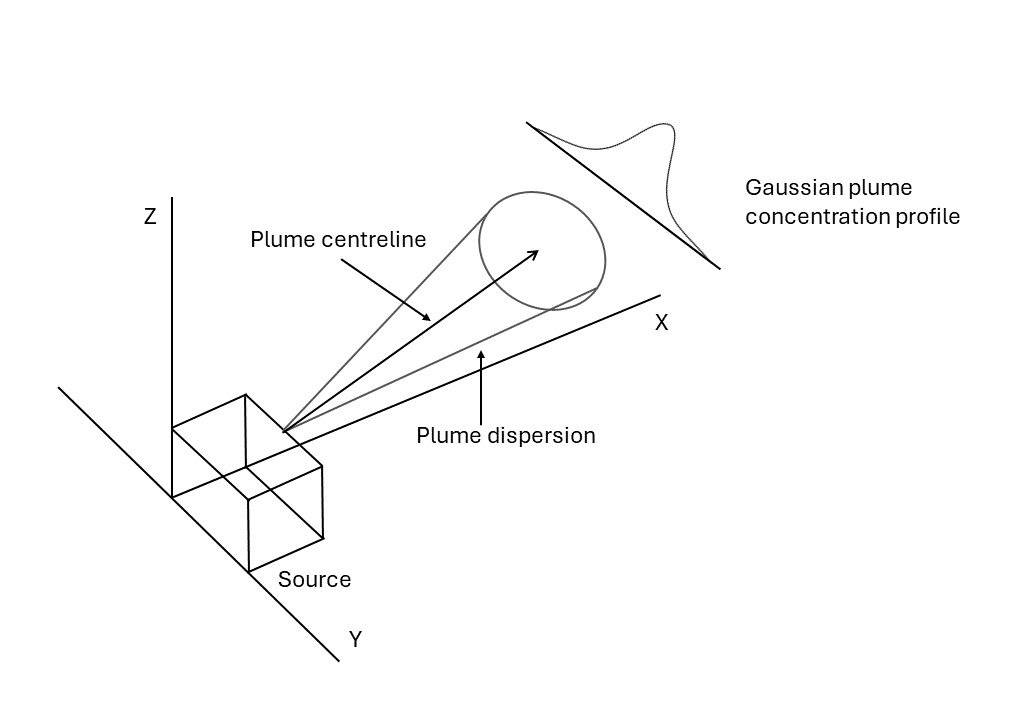
\includegraphics[width=0.8\textwidth]{Plots/gaussian plume.png}
\caption{\label{fig:gauss_plume}} Simplified representation of a Gaussian plume dispersion.  
\end{figure}

ADMS 6, developed by Cambridge Environmental Research Consultants (CERC), is a newer generation of Gaussian dispersion models. It incorporates a skewed Gaussian concentration, meaning asymmetric spatial distribution of pollutants, and atmospheric parameters that account for boundary layer conditions. The latter can vary greatly, depending on the time of the day, time of the year, and meteorology. The parameters included in ADMS 6 to simulate   for these changes are the Monin-Obukhov length, which accounts for the boundary layer height \parencite{Sathe2011ComparisonSea}. These new additions allow ADMS 6 to generate more accurate and realistic simulations of pollutant concentrations compared to simpler models.



\subsection{ ADMS Input parameters}
The ADMS 6 interface is split into 6 sections of input parameters: Setup, source, meteorology, background, grids and output.  

\subsubsection{Setup}

The setup section defines the model domain coordinate system and site-specific details. Additionally, input files can be uploaded for advanced functionalities, such as marine boundary layer conditions, as used in this study.

\subsubsection{Source}

The source section specifies the origin of simulated emissions. For oil and gas facilities, we characterise methane releases as volume sources. 

Oil and gas platforms present challenges when selecting an appropriate source type for modelling. ADMS offers several options, including point, volume, area, and jet sources. In this study, we opt to model the platforms as volume sources for several reasons.
Firstly, previous attempts at modelling similar platforms employed point sources. This approach requires defining the height, diameter, and exit velocity of the source, often mimicking a stack. However, the exit velocity in a platform scenario represents the combined velocity of all emitted compounds, including non-pollutants like water vapour, making it difficult to estimate accurately. Additionally, the precise location of the leak within the platform structure is often unknown. Research by other groups has demonstrated that variations in this parameter can significantly impact model outputs, introducing substantial uncertainty.
Methane emissions can arise from various equipment leaks, venting points, and other fugitive pathways spread across the complex PUQ facility (Figure 4).

\begin{figure}[H]
\centering
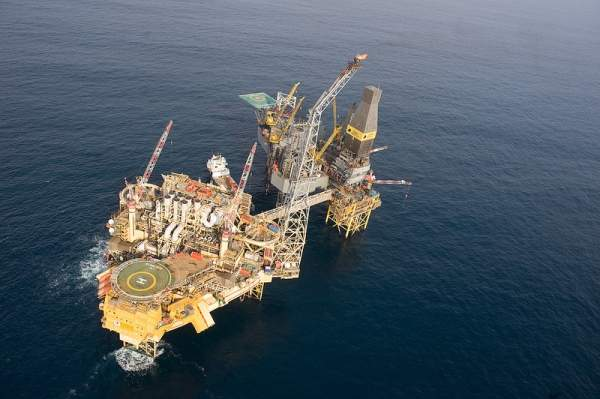
\includegraphics[width=0.8\textwidth]{Plots/Elgin-3 Picture.jpg}
\caption{\label{fig:volume source}} Elgin PUQ platform. Credit: Total Energies. 
\end{figure}

Volume sources represent well-mixed areas with vertical extent but no simulated plume rise. Essentially, the emissions are assumed to be well-distributed within a specific height range above source level, encompassing the area of the facility (Figure 5).
\begin{figure}[H]
\centering
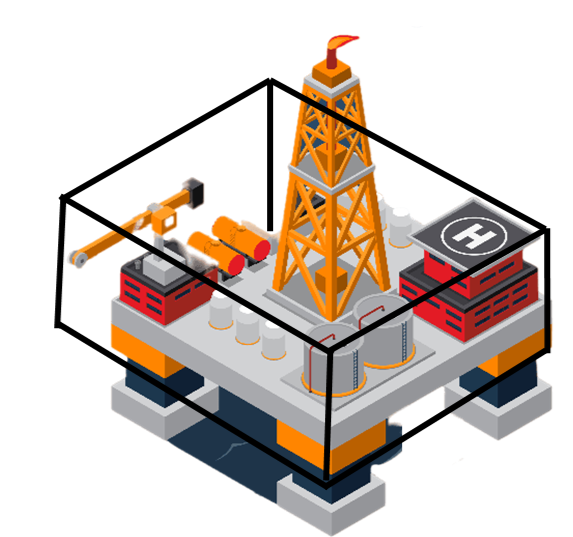
\includegraphics[width=0.4\textwidth]{Plots/rig.png}
\caption{\label{fig:volume source}} Graphic representation of a volume source for oil and gas facilities. 
\end{figure}

The size and coordinates of the Elgin PUQ facility were obtained from high resolution satellite imagery (Sentinel-2 L2A \parencite{CopernicusDataSpaceSentinel-2Data}) (Figure 6). The height of the facility was estimated by using images provided by TOTAL, and then scaling up distances from standardised structures such as the size of shipping containers to the overall height of the facility. The estimated dimensions are (103m x 80m x 25m).  The uncertainty on each axis is estimated to be approximately 10m (Table 2), therefore, the estimated volume uncertainty is 1000 m\textsuperscript{3},  0.5\% of the total volume. Given that the facility is not an exact cube, the total volume uncertainty for the source is much lager than 1000 m\textsuperscript{3}.

\begin{table}[H]
\caption{Latitudes, longitudes and estimated volume of the Elgin PUQ facility.}
\centering
\label{tab:vol_coords}
\begin{tabular}{{@{}lll@{}}}
\toprule
Latitude (degE) & Longitude (degN) & Volume ($m\textsuperscript{3}$)   \\ \midrule
57.01            & 1.836             & $206100 \pm 1000$ \\
\bottomrule
\end{tabular}
\end{table}


\begin{figure}[H]
\centering
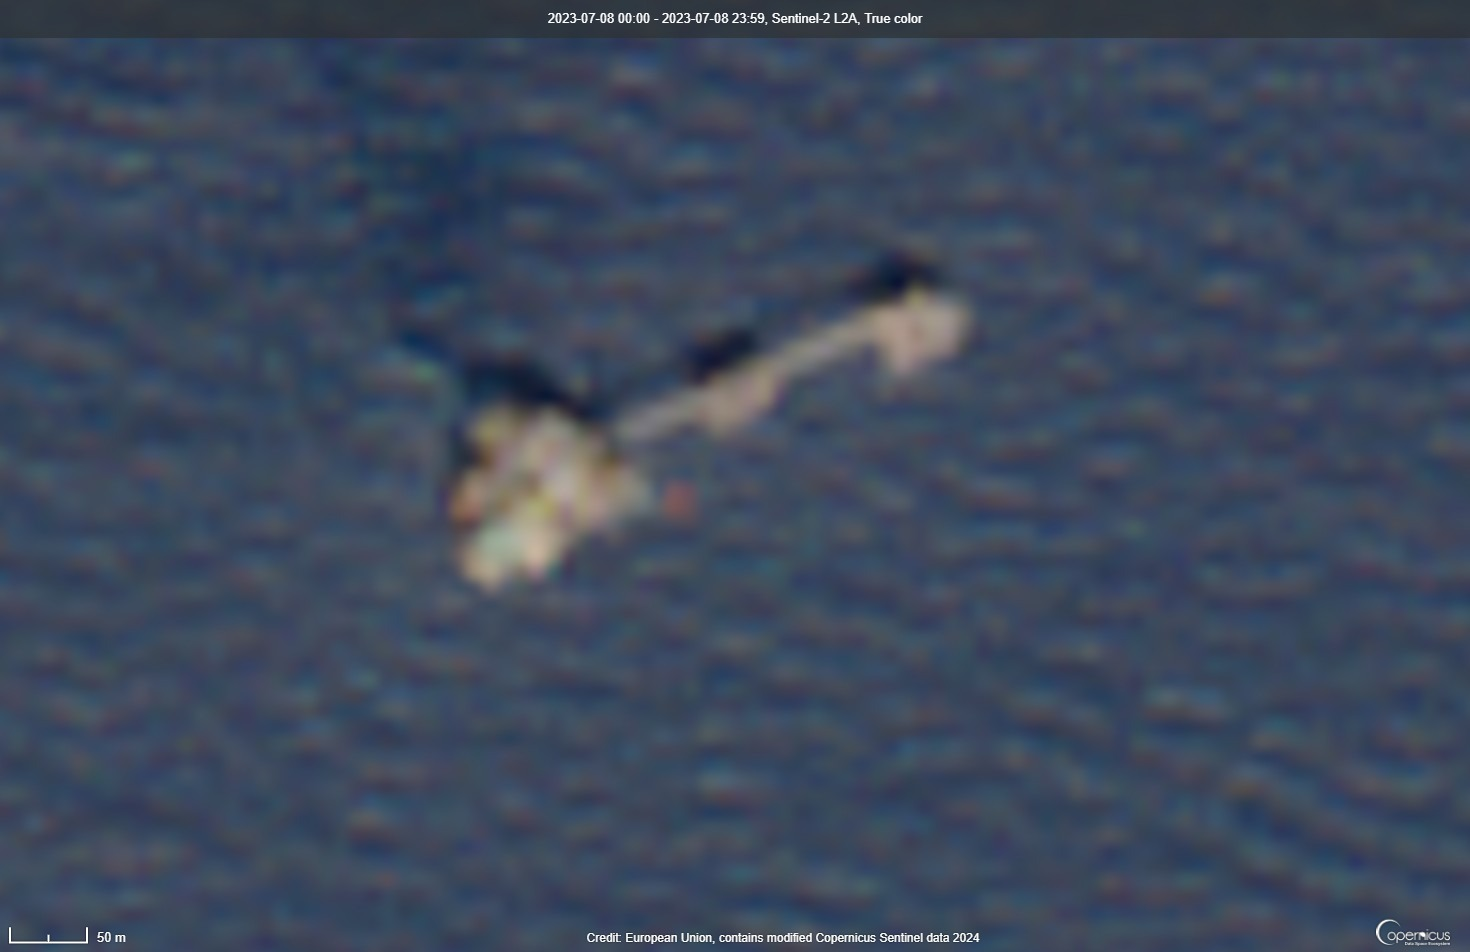
\includegraphics[width=0.8\textwidth]{Plots/2023-07-08-00_00_2023-07-08-23_59_Sentinel-2_L2A_True_color.jpg}
\caption{\label{fig:Elgin satellite}} Satellite image from Elgin PUQ facility (left), Elgin wellhead platform A (middle), and a wellhead platform B installed after the uncontrolled release, in September 2012 (right) . 
\end{figure}

After the volume source has been identified, the pollutants being emitted from it can be selected. The pollutant, methane, and its emission rate, as well as the temperature of the release are specified by the user.  

\subsubsection{Meteorology}

In the meteorology section, a .met file can be uploaded, or meteorological data can be entered manually. ADMS can read three types of meteorological data: A series of unrelated meteorological conditions, a series of hourly sequential data covering a certain period and statistical data covering a series of years. For this project, we use the hourly sequential setting and the meteorology measurements obtained from the FAAM aircraft. 

The highest resolution of meteorology data allowed in ADMS is 1h, and for the input settings used, ADMS outputs a different modelled scenario for each hour of met data provided. The meteorology variables obtained while the aircraft was flying over the source were averaged to 1h of met data, outputting a single dispersion. Meteorological variability  can be accounted for by including standard deviation parameters in the input files. However, FAAM airborne missions during the 2012 Elgin incident were no longer than 3 hours, during which meteorological parameters are often near constant, making a 1h average a suitable approach. In the flight used to test this methodology, B689,  conditions were constant throughout the mission, and thus meteorological values were averaged for the .met file (Table 3). The effect on winds in the dispersion will be discussed in sections 2.7.3 and 3.2.3.

\begin{table}[H]
\centering
\caption{Meteorogical values in .met file}
\label{tab:my-table}
\begin{tabular}{@{}lll@{}}
\toprule

Variable                & Value & Units           \\  \midrule
Temperature& 1.5   & Degrees Celsius \\
Average wind speed              & 11.9  & m/s             \\
Average wind direction          & 240   & Degrees         \\
Wind speed standard deviation & 4.35  & m/s             \\
Cloud cover             & 7     & Oktas           \\
\bottomrule
\end{tabular}
\end{table}

To improve the accuracy of model predictions, an additional input file containing data on the marine boundary layer (MBL) conditions was added. The MBL exhibits distinct properties compared to the continental  boundary layer.  One critical feature of the MBL is sea surface temperature.  Open seas and oceans exhibit significant temporal and spatial uniformity in temperature, especially within small scales \parencite[]{1988ChapterLayer}. During the flight, dropsondes launched from the FAAM aircraft measured a boundary layer height of 1.13 km \parencite[]{Lee2018FlowRelease}.

\subsubsection{Background and grid}

The background section was set to 0 to obtain methane enhancements only as an output. Model grid and resolution are determined from flight track coordinates and flying speed.The model dispersion domain is therefore limited to the domain sampled by the aircraft. This is to ease the management of large volume of high resolution output model data. The conversion from aircraft latitudinal/longitudinal coordinates system to to the model reference grid is explained in section 2.5.2. 
\subsubsection{Output}

The output section, the pollutants included in the output concentrations are determined, methane in this case. Short-term averages are selected, since only an hour of meteorological data is provided, and the time frame of the observations with the FAAM aircraft is no longer than 3  hours. This menu selection allows outputting a single-plume scenario per model run. 1s was chosen as the averaging time, the lowest time resolution possible in ADMS, considering that the aircraft observations employed in this study are also 1s time resolved. This translates into negligible plume meandering in the model results. 


\subsection{Dispersed plume enhancement calculations
}
Considering the dispersion of a plume in space within a {x, y, z} coordinate system (Figure 7), where x is the distance from the source, y the cross-wind distance from the plume centreline (horizontal dispersion), and z the plume height (vertical dispersion), we can calculate the total concentration enhancement in the plume in a yz plane at distance x from the source emission (TIE\textsubscript{yz}), by integrating concentration enhancements E(y,z) (1). 

\begin{equation}
TIE\textsubscript{yz} = \int_{z\textsubscript{min}}^{MBLH} \int_{y\textsubscript{min}}^{y\textsubscript{max}} E(y,z) \, dy \, dz
\end{equation}

The emission ratios approach in this study (section 2.1) relies on quantifying TIE\textsubscript{yz} values for co-located airborne observations and modelled dispersion.  Due to the scarcity of observations, in particular along the vertical height axis, TIE\textsubscript{yz} is calculated as follows.



Step 1: Cross-wind integrated concentration enhancements across y at height z are first calculated for each  level of cross-wind transects, by integrating concentration enhancements (E\textsubscript{z}(y))  to obtain:

\begin{equation}
IE\textsubscript{z}y = \int_{y\textsubscript{min}}^{y\textsubscript{max}} E\textsubscript{z}(y) \, dy   (ppb*m)
\end{equation}

Step 2: We then integrate all IE\textsubscript{z}y across z to obtain the total integrated enhancement across the yz plane as follows:
\begin{equation}
TIE\textsubscript{yz}  = \int_{z\textsubscript{min}}^{MBLH} IE\textsubscript{z}y(z) \, dz (ppb*m\textsuperscript{2})
\end{equation}

\begin{figure}[H]
\centering
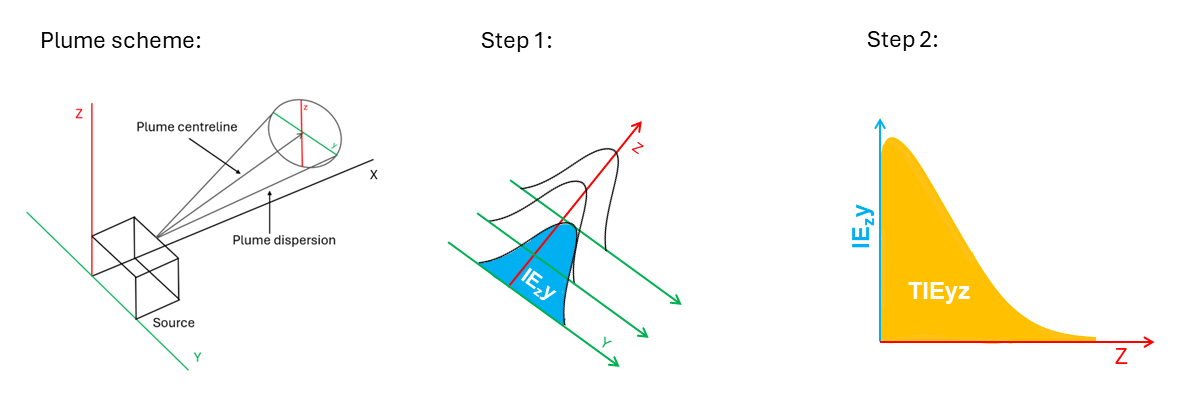
\includegraphics[width=1\textwidth]{Plots/gaussian plume calc.png}
\caption{\label{fig:volume source}} Graphic representation of dispersed plume enhancement calculations.  
\end{figure}
\subsubsection{Mission B689 data set}

FAAM observations involve cross-wind transects flown downwind of the platform at various altitudes to capture the full extent of the plume's horizontal and vertical dispersion (Figure 8).
\begin{figure}[H]
\centering
\includegraphics[width=0.8\textwidth]{Plots/b689_plume_enhancement.png}
\caption{\label{fig:volume source}} Altitude–latitude projection of the vertically stacked
downwind transects conducted in flight B689 at 5NM from the source, coloured by the CH4 enhancements.  
\end{figure}

This sampling strategy, allows for the calculation of IE\textsubscript{z}y at each flight level, which  represents the increase in pollutant concentration above background levels. Background levels are sampled upwind of the source and then subtracted from the downwind transects to obtain enhancements.  The upwind transects also confirm that no other plumes are entering the dispersion domain upwind of the identified source emitter, which would otherwise create plume overlap. 

In mission B689 data set, the methane plume was sampled at three distances from the source, 5 NM, 15 NM and 25 NM. However, the transects at 15 NM and 25 NM showed that the plume was fully mixed within the boundary layer, with similar enhancements at all altitudes  (Figure 9).

\begin{figure}[H]
\centering
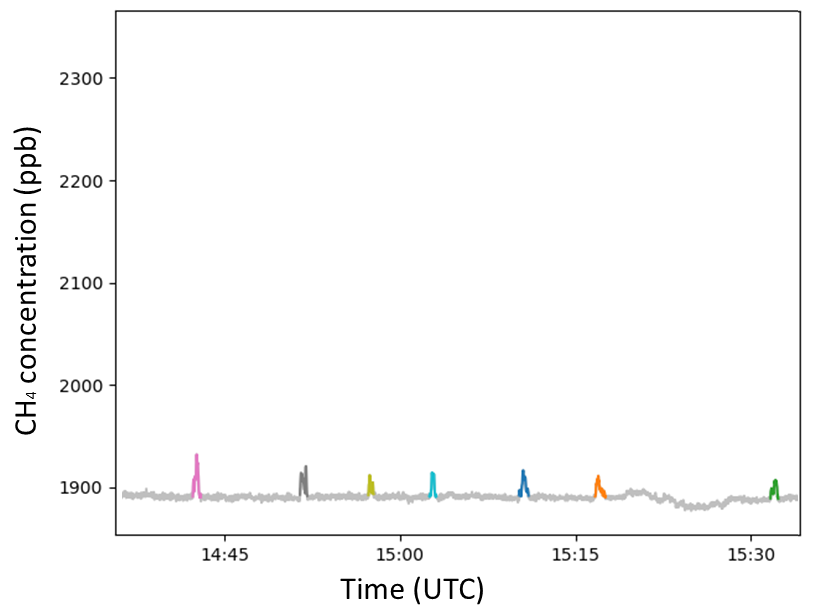
\includegraphics[width=0.8\textwidth]{Plots/peak_id_mixed_plume.png}
\caption{\label{fig:volume source}} Timescale  of CH\textsubscript{4} mixing ratios in  flight B689 at 15NM and 25NM from the source. Heights sampled range between 30 to 595m.  
\end{figure}

ADMS is a (skewed) Gaussian dispersion model, so is unsuitable to model a fully mixed MBL scenario at 15 and 25 NM. As a consequence, only the transects sampled at 5NM were used in this study (Figure 10). 

\begin{figure}[H]
\centering
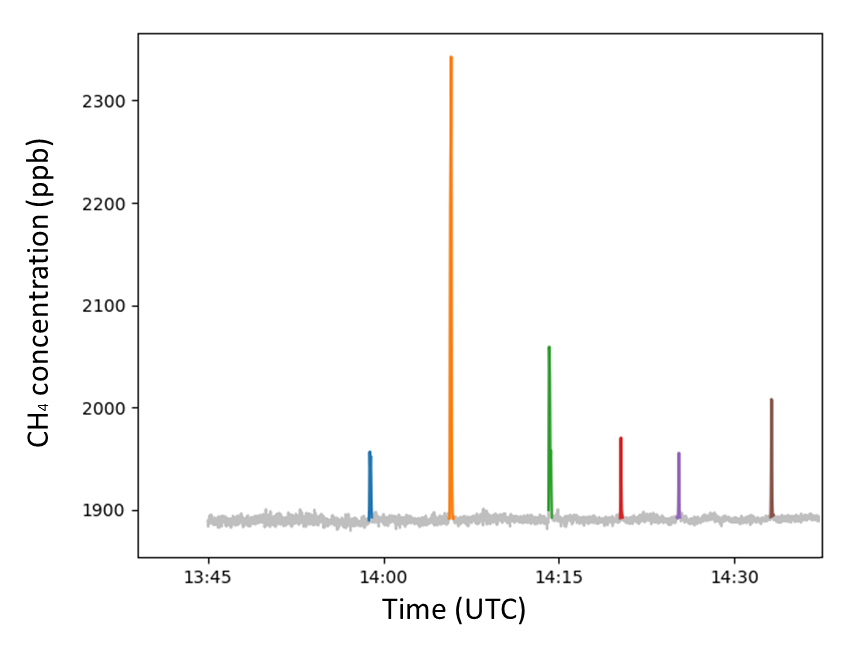
\includegraphics[width=0.8\textwidth]{Plots/peak_id_b689.png}
\caption{\label{fig:volume source}} Timescale  of CH\textsubscript{4} mixing ratios in  flight B689 at 5NM from the source.  Heights sampled range between 30 to 595m.  
\end{figure}

Further analysis involves calculating the peak area for each plume enhancement at different altitudes (IE\textsubscript{z}y)  using software developed by the FAAM Airborne Laboratory and the Wolfson Atmospheric Chemistry Laboratories \parencite{Lacy2023Acruise-peakid} . These calculated (IE\textsubscript{z}y)   are in units of ppb*s, and to convert them to ppb*m, the obtained values are multiplied by the aircraft ground speed at each altitude. 

By  plotting (IE\textsubscript{z}y) against their corresponding heights, TIE\textsubscript{yz}  can be calculated. (See Appendix A for python code).

\subsubsection{ADMS dataset}

ADMS utilises .apl files for input, and these files are typically created manually through the ADMS interface. Our methodology fixes an initial emission flux to 100g/s of methane within the ADMS input interface (section 2.6). This generates a single-modelled plume. Crucially, the model horizontal and vertical resolutions are chosen to encompass aircraft observations, ensuring comparable datasets.


Following the same analysis approach as with aircraft data, the modelled data undergo the 2-step integration to compute TIE\textsubscript{yz} enhancements.

To compare modelled and observed enhancements, the flight transects latitudes and longitudes are matched within the ADMS modelled data domain (X,Y coordinates in meters). In order to co-locate the aircraft flight track data within the ADMS modelled grid, a two-step process for spatial conversion is used. First, the Haversine formula is used to calculate the great-circle distance between each {degN latitude, degE longitude} aircraft flight data coordinates and a chosen reference point, in this case the source emitter coordinates (Elgi n PUQ). This reference point is the origin {0,0} of the ADMS model domain grid. Then, a function translates these distances into X (easting) and Y (northing) offsets relative to the reference point. By applying this 2-step conversion to every flight track coordinates, we generate new {X, Y} metre displacement from origin coordinates representing the sampled flight track within the ADMS grid, enabling spatial analysis of both datasets (See Appendix B for python script). 

Once the segments of ADMS data equivalent to the aircrafrt observations have been identified for each height, the distance between the start and end of the cross wind flight transect is identified. The modelled enhancements are plotted over this distance, and a Gaussian function fitted to calculate IE\textsubscript{z}y. This removed any potential bias arising from divergence between dispersion modelled and observed enhancements, in particular uncorrected instrumental measurement lag-time (See Appendix C for Python script) (Figure 11). 
\begin{figure}[H]
\centering
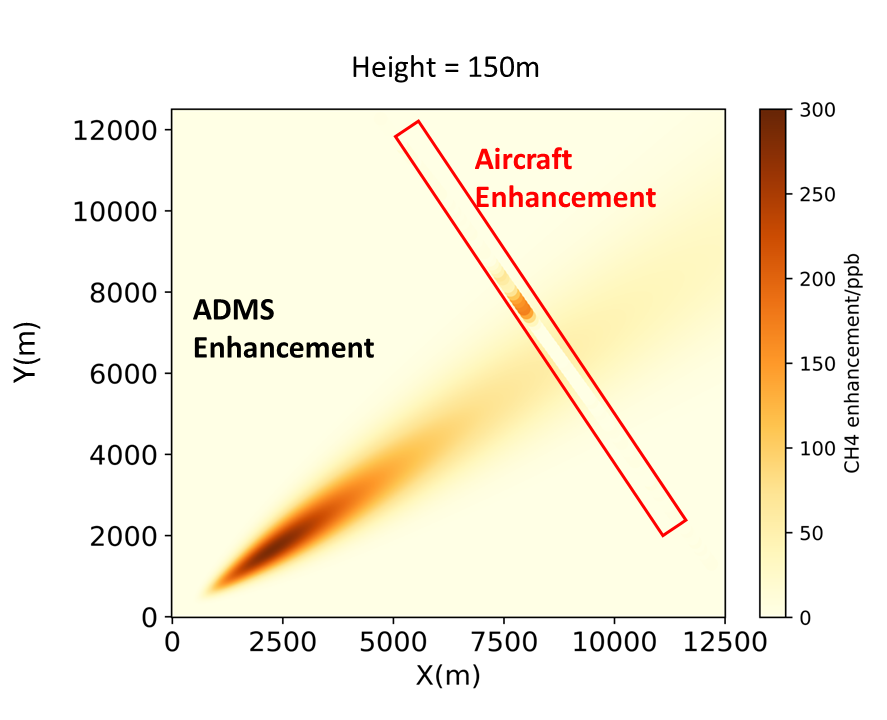
\includegraphics[width=0.8\textwidth]{Plots/adms_faam_heatmap.png}
\caption{\label{fig:volume source}} Heatmap of ADMS (black) and Aircraft enhancements (red) at a height of 150m. Colour scale: CH\textsubscript{4} enhancement (ppb).  
\end{figure}

Once IE\textsubscript{z}y of the individual heights are calculated, they are plotted against the height and a half-gaussian function is fitted. TIE\textsubscript{yz} and its corresponding error are calculated using Monte-Carlo integration (see Appendix B for python script). 

 \subsection{Flux estimation}
After TIE\textsubscript{y,z} has been calculated for both ADMS and aircraft datasets at 5NM from the source, the emission flux can be estimated. 

Given that the  TIE\textsubscript{yz} value for the ADMS datasets corresponds to an emission flux imput of 100g/s of methane , the emission flux from the source can be scaled to the airborne observed enhancements using (4).
\begin{equation}
\frac{{\text{{Aircraft TIE\textsubscript{yz}}(ppb*m\textsuperscript{2})}}*{\text{ADMS emission flux input (g/s)}}}{{\text{{ADMS TIE\textsubscript{yz}(ppb*m\textsuperscript{2})}}}} = \text{{Emission flux from source (g/s)}}
\end{equation}

The emission flux derived from this emission ratios approach could be affected by nonlinear mathematical treatments of dispersion in ADMS. The scalability aspect of ADMS dispersion calculations will be discussed in section 3.4.
\subsection{ADMS model sensitivity analysis
}
ADMS offers a wide range of input options, leading to diverse modelling approaches and assumptions. This variety can significantly impact model outputs. To study the potential effect of the model settings, a sensitivity analysis was conducted. Model input parameters were modified, and the resulting dispersion outputs were analysed to study their effect on the final flux calculation. 
\subsubsection{Source type and size
}
After having established the oil and gas facilities as volume sources, the source size needs consideration.  For this study the exact size and position of the source has to be estimated through high resolution satellite imagery, with an associated uncertainty of 1000m\textsuperscript{3}. It arises from the estimation of volume, which has an associated error of around 10m for all axis. To asses the variability of the results to this uncertainly, the model was run reducing the source by 10 metres along the x axis. 

\subsubsection{Marine Boundary layer}
The ADMS input interface has the option to add additional files (.aai). These are directly created through the ADMS interface. To successfully mimic the sampling conditions, the MBL option was used, assuming steady conditions and inputting wind speed, direction and temperature available from the FAAM aircraft. The Charnock parameter needs to be specified, which is a constant used to perform heat flux calculations as described in \cite{CambridgeEnvironmentalResearchConsultants2020ADMSGuide}. The value used is 0.08, as advised by CERC, which is representative of the conditions over the North Sea. 
The flux estimation outcomes obtained with and without the implementation of the MBL option are compared to evaluate its impact.
\subsubsection{Winds}
Wind speed and direction can significantly influence dispersion modelling results in ADMS.  We treat wind speed and wind direction in three different ways to compare results. 
For the first two methods, the model was run on a 2D grid encompassing the observation heights (30-595 m). They differ in how wind data from the aircraft measurements is incorporated. For the first method, wind speed and direction are averaged for each height transect measured and assigned to the corresponding model level in the .met file. The "height of wind measurement" variable in ADMS was also set to each modelled height. The second method used a single, overall average wind speed and direction for all model heights. This average was calculated from the  1h observation period. The "height of wind measurement" was set to each individual model height, effectively forcing the model to use the same winds throughout the domain.
The third method employed a 3D grid with domain limits defined by the observations. A single wind speed and direction, obtained from the overall average of the sampling period, was assigned. However, the "height of wind measurement" was set to the midpoint of the observed heights. This allowed ADMS to calculate a vertical wind profile based on the single wind measurement.

\newpage\section{Results and discussion}\label{res}

\subsection{Aircraft observations and near-surface considerations}
The distribution of observed IE\textsubscript{z}y enhancements against height  at 5 NM does not follow the expected vertical Gaussian distribution.  In Figure 12 we fit a log-normal function with non-zero tailing.


\begin{figure}[H]
\centering
\includegraphics[width=0.9\textwidth]{Plots/faam_IEZY.png}
\caption{\label{fig:volume source}} Vertical distribution of IE\textsubscript{z}y
(ppb*m). The red scattered points represent the calculated IE\textsubscript{z}y values for each height transect. Red line denotes log-normal fit and its corresponding uncertainty in shaded red for the Monte-Carlo method.  
\end{figure}

The low enhancement at the minimum height of 30 m is particularly surprising. The observations suggest that the plume is well mixed above 200 m due to the neutrally stratified marine boundary layer (section 3.5). Due to the poor mixing observed at the lowest 30 m altitude (low enhancement), and to avoid introducing unknown bias, TIEyz enhancements at 5 NM are calculated using Equation 3 with zmin = 75 m and zmax = 595 m (Table 4). 

By avoiding lower altitudes we aim to lower the uncertainty on flux calculations.
 
This change allows the new curve fit to be a half Gaussian function instead of a log-normal (Figure 13). Three different curve fits were created  to match the half Gaussian curve with the observed data. Since the exact altitude of the highest enhancement at 5 NM is unknown, three simulations were considered: in the first scenario, the highest enhancement from the source height of 25 m is centred at 75 m; in the second scenario, the highest enhancement rises from the source height up to an altitude of 50m; and in the third scenario, it is assumed that the highest enhancement remains at the source height of 25m without vertical movement.

\begin{figure}[H]
\centering
\includegraphics[width=0.9\textwidth]{Plots/peak_areas_faam.png}
\caption{\label{fig:volume source}}Vertical distribution of IE\textsubscript{z}y
(ppb*m) for 3 different scenarios. The pink scattered points represent the calculated IE\textsubscript{z}y values for each height transect. Three Gaussian curves are overlaid, each representing a different scenario with the centre at 25m (blue), 50m (orange), and 75m (green).  
\end{figure}

All 3 scenarios describing the vertical Gaussian dispersion of observed integrated enhancements (IE\textsubscript{z}y) offer viable treatment. 

Higher enhancements below the Elgin PUQ  deck height (25m) are improbable due to the following factors.

The uncontrolled release was characterised by very high pressure and consequently high velocity (Figure 14),  likely resulting in rapid dispersion of the gas and limited accumulation at lower levels.
\begin{figure}[H]
\centering
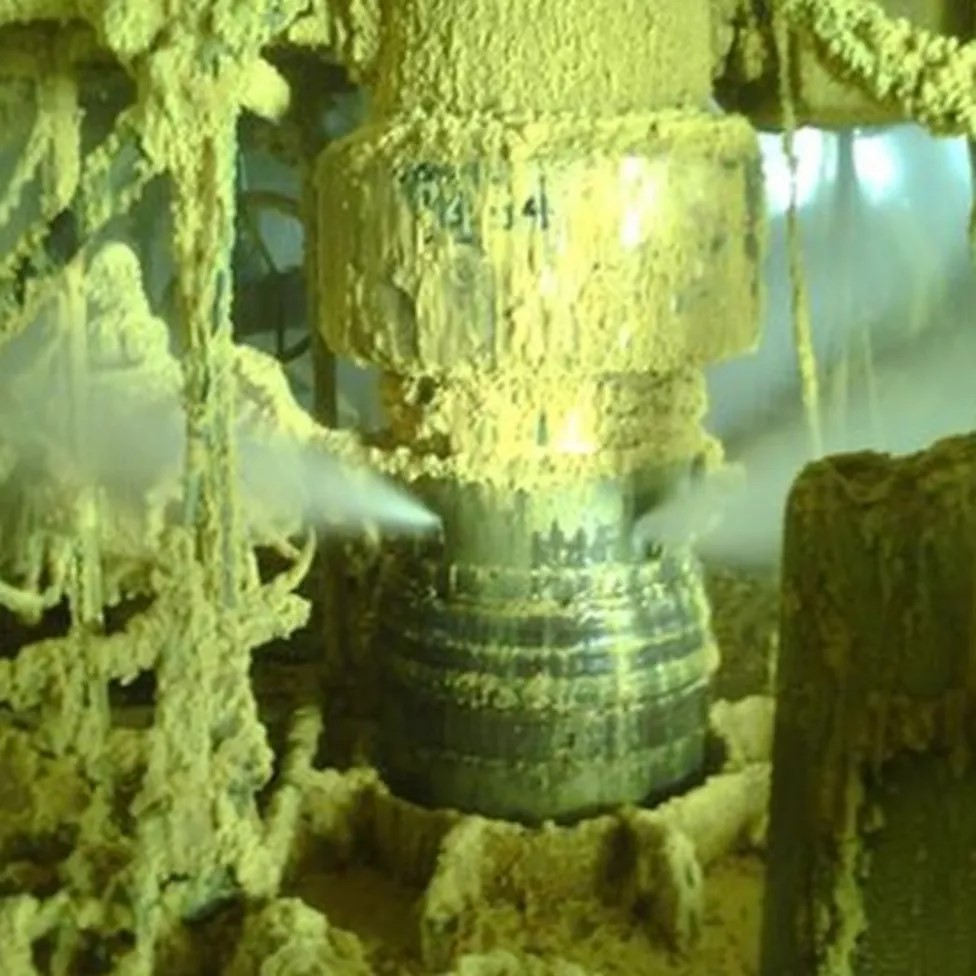
\includegraphics[width=0.4\textwidth]{Plots/wellhead.jpg}
\caption{\label{fig:volume source}Elgin wellhead leak.}  
\end{figure}


The released gas was at elevated temperatures. While the main Elgin-Franklin gas reservoirs exhibit extreme pressure and temperature conditions (around 193 \textdegree C ), the uncontrolled release originated from the shallower and comparatively cooler Hod formation secondary reservoir (165\textdegree C) \parencite{Lee2018FlowRelease}. Although buoyancy effects may have been present, the precise gas temperature at the wellhead remains unknown. For this reason, the inputed gas temperature in ADMS was ambient (Table 3). 

\cite{Lee2018FlowRelease} note that despite originating from the Hod formation at approximately 165\textdegree C, the gas likely experienced significant cooling prior to atmospheric release. This cooling is attributed to conductive heat dissipation as the gas migrates through the well casing, coupled with a temperature reduction induced by pressure drop at the leak orifice.  These combined effects would diminish the likelihood of higher enhancements closer to the ground. 


\begin{table}[]
\caption{Aircraft TIE\textsubscript{yz} values for the three proposed scenarios. }
\centering
\label{tab:faam tieyz}
\begin{tabular}{{@{}lll@{}}}
\toprule
Scenario        & TIE\textsubscript{yz} (ppb*m\textsuperscript{2}) \\ \midrule
Max fit  at 25m & 3863829    \\
Max fit  at 50m & 4642418    \\
Max fit  at 75m & 4542860  \\ \bottomrule
\end{tabular}
\end{table}

\subsection{ADMS model sensitivity analysis}
TIE\textsubscript{yz} was obtained for an emission rate input of 100 g/s in ADMS using a range of configurations to assess the sensitivity of flux calculations to factors including boundary layer options, source characteristics, model dimensionality, and wind profiles. The impact of these factors was evaluated to identify potential limitations of the ADMS model within the context of this specific case study and ultimately establish the configuration that yields the most accurate flux calculations.

\subsubsection{Volume source effect}
Using volume sources to model emissions from oil and gas platforms is effective when the fugitive nature of a leak is unknown as stated in Section 2.4.2.  By reducing the source by 10 metres along the x-axis corresponding to ~0.5\% of the total volume source defined in the initial model simulation (section 2.4.2), and keeping the rest of the model parameters constant, only a slight difference in TIE\textsubscript{yz} of  670 ppb*m\textsuperscript{3} was observed, which translates into a percentage of 0.006\%. 
The result from this sensitivity simulation is not conclusive, and the analysis should be repeated with a much larger \% change in source volume.

\subsubsection{Continental and marine boundary layer option}
TIE\textsubscript{yz} values were obtained for an emission rate input of 100g/s in ADMS under both continental and marine boundary layer (MBL) conditions, 10587458 ppb*m\textsuperscript{2} and 10810986ppb*m\textsuperscript{2} respectively (Figure 15).
\begin{figure}[H]
\centering
\includegraphics[width=0.9\textwidth]{Plots/peak_areas_faam_adms_pbl_mbl.png}
\caption{\label{fig:volume source}}Vertical distribution of IE\textsubscript{z}y
(ppb*m) for 3 different aircraft scenarios. The pink scattered points represent the calculated IE\textsubscript{z}y values for each height transect. Three Gaussian curves are overlaid, each representing a different scenario with the centre at 25m (blue), 50m (orange), and 75m (green).The red dots and line represent continental BL outputs, and blue dots and lines represent MBL outputs. 
\end{figure}

The total integrated enhancement TIE\textsubscript{yz} modelled with MBL conditions is 2\% greater than under a continental BL setup. In addition, the Gaussian shape of the dispersion in the MBL scenario mimics the observations best, with a high enhancement close to the source and a steep decrease in concentration as the height increases. Nevertheless, TIE\textsubscript{yz} values show only a marginal difference between the two scenarios. Despite the small influence of the MBL option on modelled peak areas, it will be employed in subsequent ADMS runs to accurately  represent  observational conditions.

\subsubsection{Winds}
2D Height specific wind measurements:  In this approach, a different wind speed was used for each modelled height measured by the aircraft (Figure 16) It can be observed that the modelled plume shape in red has less data points due to the limited number  of modelled heights corresponding to the number of flight transects with wind measurements. However, the modelled enhancements with height match the shape of the other 2D Uniform wind scenario (in green).

\begin{figure}[H]
\centering
\includegraphics[width=0.9\textwidth]{Plots/peak_areas_faam_adms_winds.png}
\caption{\label{fig:volume source}}Vertical distribution of IE\textsubscript{z}y
(ppb*m) for 3 different aircraft scenarios. The pink scattered points represent the calculated IE\textsubscript{z}y values for each height transect. Three Gaussian curves are overlaid, each representing a different scenario with the centre at 25m (blue), 50m (orange), and 75m (green). 3 wind scenarios modelled in ADMS are also represented. 2D  Height specific wind measurements (red), 2D Uniform wind measurements (green), 3D and single wind measurement (purple). 
\end{figure}

2D Uniform wind measurements: Utilising a single, overall average wind speed and direction for all modelled enhancements with height, this method provides a simplified representation of the wind conditions (Figure 16). The plume shape tends to exhibit Gaussian characteristics and better aligns with observed patterns by restricting ADMS from calculating its own wind profile. 

3D and single wind measurement: Employing a 3D grid with domain boundaries defined by observations, this method incorporated a single wind speed and direction derived from the overall average of the sampling period. However, by setting the "height of wind measurement" to the midpoint of observed heights, the model was able to calculate a vertical wind profile, thus capturing variations in wind throughout the vertical extent of the domain, and still exhibiting a Gaussian shape (Figure 16). As opposed to the two previous scenarios, this option shows the highest enhancements at low altitudes, very likely due to the wind profile calculations and thus predicting the lowest wind speeds closest to the source. 

Even if the difference in the obtained TIE\textsubscript{yz} values (Table 5) is only around 5\%, a few aspects need to be considered to pick the most suitable option. Even if the 2D option with height specific wind speeds accurately represents the sampling environment, the fact that the model runs are limited by the number of flight passes is not favourable. Considering this, and that the data points are in good agreement with the other wind treatment scenarios, it is more beneficial to have a larger sample size of model runs to calculate total integrated enhancements resulting in  lower associated uncertainty. 

The 2D option with uniform winds allows for a higher resolution of model outputs, however the model would be underestimating enhancements at lower altitudes, where actual wind speeds are slower.

The 3D option with a single wind speed and ADMS' own profile calculations is closest to real conditions without sacrificing model resolution, as it is able to account for lower wind speeds closer to the source. For this reason, this was the model approach used to calculate emission fluxes. 

\begin{table}[H]
\caption{ADMS TIE\textsubscript{yz} values for the three wind simulations. }
\centering
\label{tab:faam tieyz}
\begin{tabular}{{@{}lll@{}}}
\toprule
Simulation        & TIE\textsubscript{yz} (ppb*m\textsuperscript{2}) \\ \midrule
ADMS  2D Uniform wind & 8715675    \\
ADMS 2D Height specific wind & 8636417    \\
ADMS 3D Single Wind & 9120988  \\ \bottomrule
\end{tabular}
\end{table}

\subsection{Emission Flux calculation}
After the sensitivity analysis, the most optimal way to run ADMS for this study is to use volume sources to describe oil and gas fields, the MBL option and the 3D wind calculations with a single input. 
When it comes to observations, due to the uncertainty of the position of the highest enhancement in the established height range, and considering that all 3 scenarios could be equally viable, using just one scenario may yield biases in flux calculations. For this reason, the final  flux will be calculated as an average of the 3 individual fluxes derived with the three half-Gaussian fitted TIE\textsubscript{yz} values. A 1-sigma standard error for the mean flux rate is provided as uncertainty (Table 6). 
\begin{table}[H]
\caption{Emission flux calculations for the three proposed aircraft scenarios. }
\centering
\label{tab:faam tieyz}
\begin{tabular}{{@{}lll@{}}}
\toprule
Scenario        & Emission flux from source (g/s) \\ \midrule
Max fit  at 25m & 42    \\
Max fit  at 50m & 51   \\
Max fit  at 75m & 50  \\ \bottomrule
Average flux & $48\pm2$
\end{tabular}
\end{table}
Thus, final flux estimation is  $48\pm2$  g/s.  

\subsection{ADMS source strength scalability}
One potential limitation of the emission ratio approach for deriving flux rates is relying on the scalability of the source flux strength to its corresponding modelled total integrated enhancement at 5 NM, TIE\textsubscript{yz}. This scalability relies on the ADMS model dispersion equations using linear transformations. Since we do not have this model insight, we assess this scalability by re-initiating the ADMS model with the emission flux derived by our emission ratio methodology as a new input. The aim is to check the new modelled IE\textsubscript{z}y values, the total integrated enhancement TIE\textsubscript{yz} and derive again the emission flux using equation (4) . Results revealed a TIE\textsubscript{yz} of 4640884 ppb*m\textsuperscript{2} for the modelled dispersion,  with emission flux value of $46 \pm 3$ g/s (Figure 17). The difference between this new value and the input flux is 2 g/s which falls within our uncertainty. This suggests the scalability of the model dispersion  calculations is mathematically robust, confirming the suitability of this method for flux calculations.

\begin{figure}[H]
\centering
\includegraphics[width=0.9\textwidth]{Plots/peak_areas_faam_adms_calcflux.png}
\caption{\label{fig:volume source}}Vertical distribution of IE\textsubscript{z}y
(ppb*m) for 3 different aircraft scenarios. Three Gaussian curves are overlaid, each representing a different scenario with the centre at 25m (blue), 50m (orange), and 75m (green). IE\textsubscript{z}y values for the ADMS model run with the calculated flux as an input (blue) are also represented. 
\end{figure}

\subsection{Comparison to mass balance methodology}
In \cite{Lee2018FlowRelease}, two variants of the mass balance methodology were used to calculate emission fluxes for mission B689. The first method, Gaussian fitting concentrations in the vertical, was applied to observations made at 5 NM downwind of the Elgin platform.  At this distance the plume enhancements decreased up to 595 m altitude as reported in section 2.5.1.  This is consistent with methane not being mixed through the full depth of the MBL. A stable inversion layer was confirmed just above 1 km altitude by two radio dropsondes launched by FAAM at 13:00 and 16:00 UTC before the aircraft entered and exited the task area. 

The neutrally stratified conditions found in the MBL below the capping  inversion layer were ideal to apply \cite{Lee2018FlowRelease}’s second mass balance methodology for a fully mixed layer, at downwind distances of 15 and 25 NM, using a mixing height of $1.13 \pm 0.1$ km.  Further downwind of the Elgin PUQ, observations confirmed uniform methane enhancements from 35 up to 590 m altitude as shown in sections 2.5.1, 3.1.

These methods resulted in two sets of mass balance values (Table 7), and show a good agreement within 5\% for both methods.

\begin{table}[H]
\caption{Emission flux values calculated by \cite{Lee2018FlowRelease} with the mass balance methodology and by this study at different distances from the source.} 
\centering
\label{tab:faam tieyz}
\begin{tabular}{{@{}llll@{}}}
\toprule
Downwind distance from PUQ, NM              & 5         & 15        & 25       \\ \midrule
Method 1, Gaussian vertical fit flux, g/s & $550 \pm 710$ & n/a       & n/a      \\
Method 2, fully mixed MBL flux, g/s       & n/a       & $590 \pm 210$ & $580 \pm 70$ \\
This study, ADMS derived flux, g/s        & $48\pm6$& n/a       & n/a  \\ \bottomrule
\end{tabular}
\end{table}

Considering the results of the sensitivity analysis, the total combined uncertainty is 13\% which corresponds to 5\% from the wind treatment, 4\% for the model scalability and 4\% for the vertical integration of observed enhancements. 
When comparing the flux value obtained in our study with mass balanced estimated fluxes from \cite{Lee2018FlowRelease}, we find a significant difference of a factor of 10. Various factors were explored in the sensitivity analysis, including the source's location and size, marine boundary layer conditions, and wind treatment, which did not significantly affect the final derived flux. 
One potential explanation worth further investigation is the lack of exit velocity, which could lead to poorly dispersed enhancements in the vertical. This hypothesis could be tested by adjusting the representation of oil and gas platforms. An option to include exit velocity in ADMS is by defining oil and gas facilities as area sources, although this adjustment may introduce bias in its estimation.

Alternatively, employing inverse modelling is an option to compare flux calculations using ADMS with those derived from emission ratios. By evaluating different ADMS scenarios with different emission flux inputs against actual FAAM observations, the scenario with the best fit enhancement can be identified, and thus infer the emission flux from the model input values. However, given the good model's scalability demonstrated in section 3.4, minimal variation in results is anticipated.
To investigate the origin of the unexpected flux underestimation, similar observational datasets with corresponding published mass balance flux values should be analysed, to determine if calculated values using this ADMS methodology improve. 

The source volume is likely to be the main cause for the lower flux estimate.  Since the conclusion of the modelling simulations, we inspected the northerly offset of the observed methane enhancements compared to the modelled dispersion as showed in Figure 11.  It became apparent that the only explanation is the mis-location of the source.  This was later confirmed by realising that the wellhead platform (A), as showed in the satellite picture in Figure 6, was the actual source location of gas leak.  By using the Elgin PUQ, we believe that the source volume was overestimated by a significant margin.  The sensitivity simulation for the source volume (Section 3.2.1) did not yield a conclusive result as the simulated volume change was too marginal (0.5\%).  

\subsection{Limitations of ADMS in this case study}
During the course of this project, several limitations of ADMS were identified. Firstly, the model requires significant computational power, primarily due to the size and high resolution of the model domain. 

Secondly, a notable drawback specific to this study is ADMS’ inability to cope with neutral boundary layer conditions, when rapid horizontal and vertical dispersion is expected into a fully mixed layer. The meteorological conditions during B689 were less favourable to applying our methodology for further downwind conditions, and may well have been affected at the nearest operational distance for the FAAM aircraft (5 NM exclusion zone enforced during the Elgin incident).  One potential solution to address this limitation could involve incorporating additional variables into the MBL input options of ADMS to better simulate mixed conditions, such as the reciprocal of Monin-Obukhov length.

\section{Conclusion}

We estimated methane emission fluxes from the uncontrolled gas release of the Elgin offshore platform in 2012 using a combination of airborne measurements from the FAAM Airborne Laboratory and atmospheric dispersion modelling with ADMS 6.

The adoption of the emission ratio approach over traditional mass balance methodologies provided the opportunity to independently assess emission fluxes. Thanks to FAAM’s high accuracy methane and meteorological airborne measurements this study benefited from a high-resolution characterisation of the plume dispersion to validate modelled simulations.

The use of ADMS provided a powerful tool for simulating pollutant dispersion. Our sensitivity analysis explored the influence of model input parameters, such as source characterisation, boundary layer conditions, and wind profiles, highlighting the importance of careful consideration in model setup and interpretation of results. We proved that for an optimal simulation of conditions, volume sources should be used to model oil and gas assets, and their dimensions can be estimated from satellite images. We also showed that the ADMS 6 marine boundary layer scheme, which calculates surface roughness and heat flux over the sea, should be enabled to improve modelled dispersion in off-shore conditions. The analysis for the treatment of winds in ADMS 6 demonstrated that the 3D grid with a single wind measurement provides a better representation of real conditions. 

At the lowest altitude (30 m) and shortest downwind distance from the Elgin PUQ (5 NM) during mission B689, the vertical profile of measured enhancements did not follow the modelled Gaussian enhancements.  To reduce potential bias when scaling integrated observed and modelled enhancements, we initiated their vertical integration from the altitude of maximum observed enhancement (75 m).  The uncertainty associated with this treatment was evaluated by simulating three vertical half-Gaussian fits and estimated at 5\%.

After optimising the ADMS 6 model input parameters and the cross-wind and vertical integration of modelled and observed enhancements, this study estimates a methane emission flux rate of $48 \pm 6$ g/s for mission B689.  

The ADMS6 flux scalability was checked for potential bias from non-linear mathematical transformations and confirmed a potential error of 4\%.

The comparison of our flux estimations with those derived from mass balance methodologies using the same dataset revealed a difference of a factor of 10, suggesting the need for further investigation into model assumptions and parametisations, including volume source uncertainty, exit velocities, and inverse modelling. 

Despite these limitations, the ADMS model remains a highly flexible tool for analysing scenarios like the one investigated in this study. However, it's essential to bear these limitations in mind when designing similar studies in the future.

 
\newpage\printbibliography

\newpage\appendix
\section{Calculate TEI\textsubscript{yz} for airborne observations}
\lstset{
    language=Python,
    basicstyle=\ttfamily,
    keywordstyle=\color{blue},
    commentstyle=\color{purple},
    stringstyle=\color{red},
    breaklines=true,
    showstringspaces=false,
    numbers=left,
    numberstyle=\tiny,
    numbersep=10pt,
    tabsize=4,
    frame=tb
}

\begin{lstlisting}
import datetime
import pandas as pd
import numpy as np
from acruisepy import peakid
import matplotlib.pyplot as plt 
from scipy.optimize import curve_fit
from scipy.integrate import quad 
from scipy.stats import sem 


#fix timestamps and index

df = pd.read_csv("b689_fgga.csv", header=[0], parse_dates=True, index_col=0,
   date_parser=lambda x: datetime.datetime.strptime(x, "%d/%m/%Y %H:%M"),)

df=df.loc[df.index>df.index[0]]
df=df.loc[df.index<df.index[-1]]
a = pd.date_range(start=df.index[0], end=df.index[-1]+datetime.timedelta(seconds=59), freq='s')
df.index=a

#filter by time to 5NM

start_time = datetime.datetime(2012, 4, 3, 13, 45, 0)
end_time = datetime.datetime(2012, 4, 3, 15, 45, 0)
df = df.loc[start_time : end_time]

#select only methane colum and delete calibration data 
ch4= df['CH4']

ch4.loc[df['CH4_Flag'] >1] = np.nan

#save in a csv

ch4.to_csv('fgga_b689_fixed.csv')

#run peak ID 

#yellow line(plume threshold)x:limit to detect plume
#blue line (plume starting):where plume starts once it is detected
bg = peakid.identify_background(ch4, bg_sd_window=3, bg_sd_threshold=0.3, bg_mean_window=116)
#peakid.plot_background(ch4, bg, plume_sd_threshold=10, plume_sd_starting=0.5)

#calculates IEzy
plumes = peakid.detect_plumes(ch4, bg, plume_sd_threshold=10, plume_sd_starting=0.5, plume_buffer=20)
#peakid.plot_plumes(ch4, plumes)

#save areas in a df

ch4_areas = peakid.integrate_aup_trapz(ch4 - bg, plumes, dx=0.1)


#select plumes close to the source where plume was gaussian 

ch4_areas_gauss = ch4_areas.head(6)


#heights from elgin paper (approximated form core data)
heights= [30, 75, 150, 220, 295, 595]
speed =[104.986, 106.465, 100.495, 106.927, 109.417, 107.7]
#make dataset with height annd area 

ch4_areas_gauss['height'] = heights
ch4_areas_gauss['speed'] = speed

ch4_plot2 = ch4_areas_gauss[["area", "height", 'speed']]
ch4_plot2['area_s'] =  ch4_plot2['area']*ch4_plot2['speed']
ch4_plot = ch4_plot2 [["area_s", "height"]]

#reindex

ch4_plot.index = range(1, len(ch4_plot) + 1)


xdata, ydata = np.asarray(ch4_plot['height']), np.asarray(ch4_plot['area_s'])


# define log normal function
def log_normal(x, yo, A, xo, width):
    return yo + A * np.exp(-(np.log(x/xo)/width)**2)

# initial guess parameters
p0 = [40, 272, 80, 0.57]

# fit the data
popt, pcov = curve_fit(log_normal, xdata, ydata, p0=p0)

yo, A, xo, width = popt
perr = np.sqrt(np.diag(pcov))

yo_err, A_err, xo_err, width_err = perr



min_limit = np.min(xdata)
max_limit = np.max(xdata)

def integrand(x, yo, A, xo, width):
    return log_normal(x, yo, A, xo, width)
#  integrand function
def monte_carlo_integration(func, params, param_errors, x_min, x_max, num_samples=1000):
    integral_values = []
    for _ in range(num_samples):
        sampled_params = np.random.normal(params, param_errors)
        integral_value, _ = quad(func, x_min, x_max, args=tuple(sampled_params))
        integral_values.append(integral_value)
    return np.mean(integral_values), np.std(integral_values)

fit_params = popt
fit_errors = perr


#calculate TIEyz
integral_value_FAAM, integral_error_FAAM = monte_carlo_integration(integrand, fit_params, fit_errors, min_limit, max_limit)


\end{lstlisting}
\section{Translate aircraft coordinates to ADMS grid}
\begin{lstlisting}
import math
import pandas as pd
import datetime 
import matplotlib.pyplot as plt
from mpl_toolkits.mplot3d import Axes3D
import numpy as np

#read file with fgga data, lat, lon and height

df =pd.read_csv('fgga_core_b689.csv', header=[0], parse_dates=True, index_col=0,)
#adjsut for sampling time
start_time = datetime.datetime(2012, 4, 3, 13, 45, 0)
end_time = datetime.datetime(2012, 4, 3, 14, 40, 0)
df = df.loc[start_time : end_time]

#delete turns data
df = df.loc[(df['LON_GIN'] >= 1.5) & (df['LON_GIN'] <= 2)]
df = df.loc[(df['LAT_GIN'] >= 56.90) & (df['LAT_GIN'] <= 57)]

#define functions that convert FAAM lats and lons to x and y coordinates with reference to the coordinates 
    #of the source, the reference point (0,0)
    
def haversine(lat1, lon1, lat2, lon2):
    R = 6371000  #radius of the Earth in meters
    phi1 = math.radians(lat1)
    phi2 = math.radians(lat2)
    delta_phi = math.radians(lat2 - lat1)
    delta_lambda = math.radians(lon2 - lon1)
    
    a = math.sin(delta_phi/2) * math.sin(delta_phi/2) + \
        math.cos(phi1) * math.cos(phi2) * \
        math.sin(delta_lambda/2) * math.sin(delta_lambda/2)
    c = 2 * math.atan2(math.sqrt(a), math.sqrt(1-a))
    d = R * c
    
    return d

def latlon_to_xy(lat, lon, ref_lat, ref_lon):
    # reference point
    ref_x = haversine(ref_lat, ref_lon, ref_lat, lon)
    ref_y = haversine(ref_lat, ref_lon, lat, ref_lon)
    
    # target point
    x = haversine(ref_lat, ref_lon, ref_lat, lon)
    y = haversine(ref_lat, ref_lon, lat, ref_lon)
    
    return x, y

# reference point: (coordinates of the source)
ref_lat = 57.011046
ref_lon = 1.836386

#convert rows of df from lat lon to x y 
df['X'], df['Y'] = zip(*df.apply(lambda row: latlon_to_xy(row['LAT_GIN'], row['LON_GIN'], ref_lat, ref_lon), axis=1))

# calculate max and min values for X and Y
max_x = df['X'].max()
min_x = df['X'].min()
max_y = df['Y'].max()
min_y = df['Y'].min()

# create a dictionary for the results
maxmin_dict = {
    'X': {'max': max_x, 'min': min_x},
    'Y': {'max': max_y, 'min': min_y}
}

# create a DataFrame from the dictionary
max_min_df = pd.DataFrame(maxmin_dict)

df.reset_index(drop=True, inplace=True)
df = df.iloc[:, 2:]

df.to_csv('fgga_b689_x_y.csv')
\end{lstlisting}
\section{Calculate TIE\textsubscript{yz} for ADMS dataset}

\begin{lstlisting}
# read aircraft data
df_fgga2= pd.read_csv("fgga_b689_x_y.csv", header=0, index_col=0)


#degine gaussian function 
def gaussian(x, a, b, c):
    return a *np.exp(-((x-b)**2)/(2*c**2))

#define adms_peak area function
def ADMS_peak_area(filename):
    #read_.gst file
    df_adms= pd.read_csv(filename, header=0)
    #rename methane column
    df_adms.rename(columns={df_adms.columns[-1]: 'CH4'}, inplace=True)
   
    df_fgga = df_fgga2.loc[(df_fgga2['HGT_RADR'] > 280) & (df_fgga2['HGT_RADR'] <= 350)]
    #filter only useful columns
    df_fgga = df_fgga.filter(['X','Y','CH4'])
    #correct for background
    df_fgga['CH4'] = df_fgga.CH4 - 1889.0479508196722 # substract background concentration
    #interpolate adms methane data so that it matches faam coordinates. gives ch4 adms enhancements just for faam coordiantes(DAVE)
    adms_interpolated = griddata((df_adms['X(m)'], df_adms['Y(m)']), df_adms.CH4,(df_fgga.X, df_fgga.Y))
    #calculate the distance of the faam transect with pythagoras(dave)
    x = df_fgga.X
    y = df_fgga.Y
    dist_series= (((x - x.shift())**2 + (y - y.shift())**2)**0.5).cumsum().fillna(0)
    #turn dist into an array
    dist = np.array(dist_series, dtype=float)
    #calculate max methane conc
    max_index = np.argmax(adms_interpolated)

    #find corresponding distance to max ch4 value for better fit 
    distance_at_max_ch4 = dist[max_index]
    #parameters correspond to width, mean, and sd of the initial gaussian fit ans are guesses
    p0=[6000, distance_at_max_ch4,1000]
    fit, cov = curve_fit(gaussian, dist, adms_interpolated, p0=p0)

    a, b, c = fit
    #establish limits on the x axis for the integral
    min_limit_dist = np.min(dist)
    max_limit_dist = np.max(dist)
    
    #define integral function for gaussian function 

    def integrand(x):
        return gaussian(x, a, b, c)
    #integreate gaussian function 
    int_gauss_result, int_error = quad(integrand, min_limit_dist, max_limit_dist)
    #ADMS_peak_area returns the peak area for a single peak ant a single height and the error 
    return int_gauss_result, int_error

    
#directory that contains folders with the emssion flux input as folder names
#inside each folder there are different .gst files (ADMS outputs) for each height sampled by faam data
directory_1 = "D://adms_b689_report//flux_folders//winds_different_mbl"


# glob all the folders
flux_folders = os.listdir(directory_1)
#empty lists for flux, total peak area for each flux, and each error
fluxes = []
ints = []
errs = []

# interate through each folder 
for folder in flux_folders:
    #store flux value as an integer from folder name 
    flux = int(folder) 
    #add value to fluxes list for each iteration 
    fluxes.append(flux)
    #direcotry inside the folder where all the .gst files are 
    directory_2 = directory_1 + "//" +str(flux) + "//"
    gst_files = glob.glob(directory_2 + "*.gst") 
    gst_files=sorted(gst_files, key=lambda x:int(x.split('_')[-1].split('m')[0]))
        
    
    
    #create empty lists for peak areas for single peaks at different heigts
    heights = []
    peak_areas = []
    peak_errors = []
    
    # itnerate through each file in the folder.each file corresponds to a height contained in the filename
    for filename in gst_files:
        #calculate peak area (gaussian) and error for each height adnd add them to the list 
        peak_area, peak_error=ADMS_peak_area(filename)
        peak_areas.append(peak_area)
        peak_errors.append(peak_error)
        #extract height value from filename and add it to the list
        height = int(filename.split('_')[-1].split('m')[0]) 
        heights.append(height)
            
    #after loop you have 3 lists, with heights, peak areas and peak errors for a single folder(flux) (similar to peak ID data)
    height_area_results = {'heights': heights, 'peak_area': peak_areas, 'peak_area_error': peak_errors}

    # convert the dictionary to a dataframe 
    height_area_results = pd.DataFrame(height_area_results)
    height_area_results.to_csv('100_mbl_diff winds_height_area_results.csv')
df_2 =pd.read_csv('100_PBL_samews_results.csv', index_col=0, header=0)
x_data_adms_2 = np.array(df_2['heights'])
y_data_adms_2 = np.array(df_2['peak_area'])

# define half gaussian
def half_gaussian(x,a1,b1,c1):
   return a1*np.exp(-((x-b1)/c1)**2)

guess =(25658, 69.2191,479.5105)

fit_1,err_1 = curve_fit(half_gaussian, x_data_adms_1, y_data_adms_1, p0=guess)

a1_1,b1_1,c1_1 =fit_1
    
perradms_1 = np.sqrt(np.diag(err_1))

def integrand(x,a1,b1,c1):
    return half_gaussian(x,a1,b1,c1)

# define  monte carlo 
def monte_carlo_integration(func, params, param_errors, x_min, x_max, num_samples=5000):
    integral_values = []
    for _ in range(num_samples):
        sampled_params = np.random.normal(params, param_errors)
        integral_value, _ = quad(func, x_min, x_max, args=tuple(sampled_params))
        integral_values.append(integral_value)
    return np.mean(integral_values), np.std(integral_values)


# integration limits
x_min = 30
x_max = 595

# perform Monte Carlo integration
integral_value_adms_1, integral_error_adms_1 = monte_carlo_integration(integrand, fit_1, perradms_1, x_min, x_max)
\end{lstlisting}



\end{document}